%%%%%%%%%%%%%%%%%%%%%%%%%%%%%%%%%%%%%%%%%%%%%%%%%%%
%
%  New template code for TAMU Theses and Dissertations starting Fall 2012.  
%  For more info about this template or the 
%  TAMU LaTeX User's Group, see http://www.howdy.me/.
%
%  Author: Wendy Lynn Turner 
%	 Version 1.0 
%  Last updated 8/5/2012
%
%%%%%%%%%%%%%%%%%%%%%%%%%%%%%%%%%%%%%%%%%%%%%%%%%%%

%%%%%%%%%%%%%%%%%%%%%%%%%%%%%%%%%%%%%%%%%%%%%%%%%%%%%%%%%%%%%%%%%%%%%%
%%                           SECTION I
%%%%%%%%%%%%%%%%%%%%%%%%%%%%%%%%%%%%%%%%%%%%%%%%%%%%%%%%%%%%%%%%%%%%%


\pagestyle{plain} % No headers, just page numbers
\pagenumbering{arabic} % Arabic numerals
\setcounter{page}{1}


% \renewcommand*{\thefootnote}{\fnsymbol{footnote}}
\chapter[\uppercase{Introduction}]{\uppercase{Introduction}}
% \symbolfootnote[1]{Reprinted with permission from ``Introduction: The Importance of Research'' by AUTHOR et al., 2015. The Astrophysical Journal, Volume XYZ, Issue X, article id. XY, XY pp., Copyright 20XX by the American Astronomical Society.} }
% \renewcommand*{\thefootnote}{\arabic{footnote}}
% \setcounter{footnote}{0}

This thesis focuses on how we may use upcoming large-area sky surveys to better understand galaxy clusters in a cosmological context. It covers a broad range of topics from galaxy clusters, to planning and observing, cosmology, probability and statistics, numerical simulations, data reduction, and machine learning. As such, the work presented here stands at the emerging intersection of astronomy and data science.

To begin, we introduce many of the basic concepts needed to understand the relevance of this thesis. While this overview is certainly not comprehensive, it should provide the basic knowledge to follow the remaining discussion. The following two chapters constitute the bulk of our analysis, and can be thought of as a theoretical study and a practical test of the theory. We conclude with a look to the future and how this thesis might be extended to other pressing issues in astronomy today.

But first, we begin by discussing what clusters of galaxies are, how they are deeply related to the cosmological parameters of the Universe, and how we go about studying them. We provide a brief introduction, through example, to some of the key concepts of machine learning, and conclude with a discussion of the importance of this work to set the stage for this thesis.

\section{Galaxy Clusters}
Clusters of galaxies are large gravitationally bound, highly over-dense, systems of galaxies. A collection of galaxies (now known to be the Virgo Cluster) was first documented by Charles Messier in 1781 as entry 91 in his catalog, and their study has been active ever since. The place of galaxy galaxy clusters in the canon was solidified when Edwin Hubble proved their constituent nebulae were not bound to the Milky Way \citep{Hubble1926}, but were collections of stars similar to the Milky Way. Work to understand their nature and origin began in ernest when \cite{Hubble1931} used the virial theorem and the galaxy velocities in the centers of the Virgo \citep{Smith1936} and Coma \citep{Zwicky1933} clusters to derive their masses. Fritz Zwicky measured the average velocity of the Coma Cluster galaxies with respect to one another to be 977 \kms, leading to a virial mass estimate of $3.3 \times 10^{15}$ \Msol. After comparing this mass estimate to the total luminosity from the cluster member galaxies, he found a mass-to-light ratio of approximately 660:1. This led Zwicky to theorize the existence of large amounts of non-luminous matter and coin the term ``dark matter'' (DM), which we still use today.  

Some controversy surrounds what exactly constitutes a ``galaxy cluster,'' as small associations of galaxies are often referred to as ``groups''. \cite{Abell1958} defines a ``richness'' parameter as the number of cluster member galaxies with brightnesses between the magnitude of the third brightest member, $m_3$, and $m_3 + 2$. Galaxy associations with a richness of 30 or more are routinely referred to as rich clusters and those structures with richness between three and 30 are classified as poor groups. Because this definition is far from universal, we will not make a distinction in this thesis, any bound system of galaxies we refer to as a cluster, and we will use the richness as a parameter that correlates with total cluster mass.

\begin{figure}[!ht]
	\begin{center}
		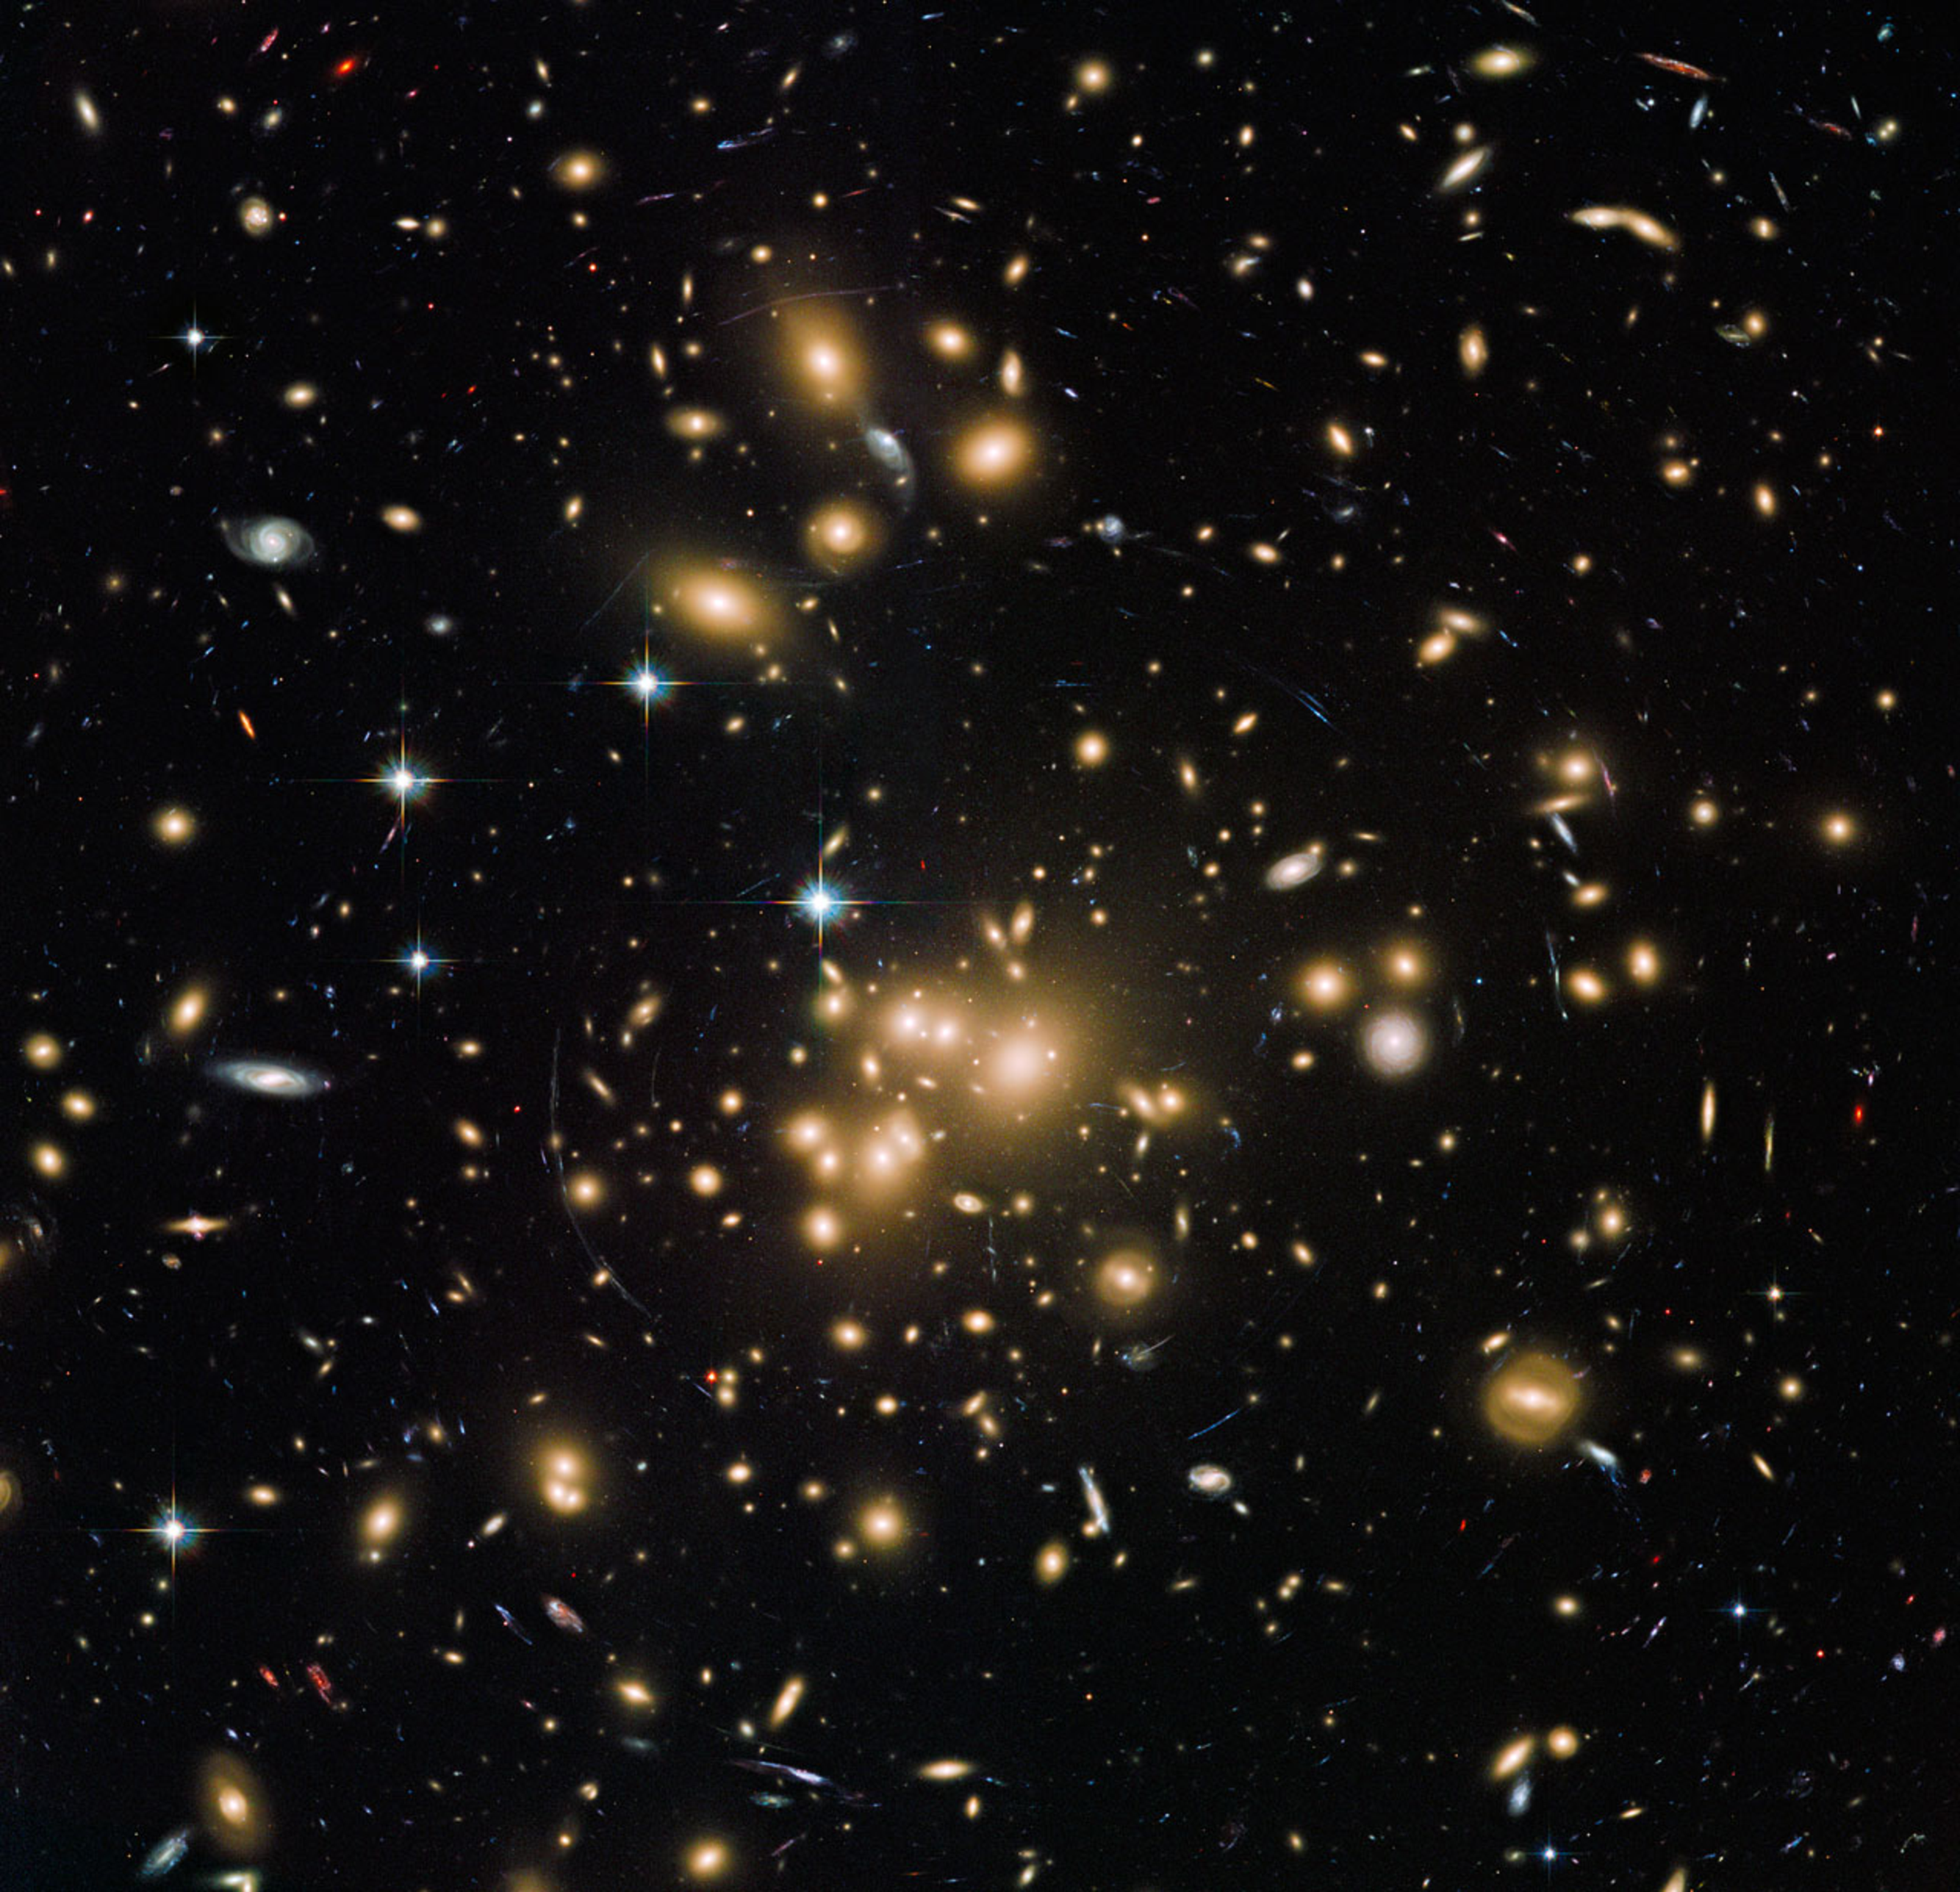
\includegraphics[height=0.5\textheight]{figures/abell1689_hubble.pdf} 
	\end{center}
	\caption[Hubble Space Telescope image of galaxy cluster Abell 1689.]{Hubble Space Telescope image of galaxy cluster Abell 1689. Many of the galaxies visible are associated with the cluster. Not visible is the ICM or the larger DM halo which constitues the majority of the cluster mass. Credit: ESA/Hubble [CC BY 3.0]}
	\label{fig: abell1689_hubble} 
\end{figure}

Modern astronomy catalogues the composition of galaxy clusters in three main parts: the member galaxies, the hot inter-galaxy gas, and the surrounding DM. In optical and near-infrared wavelengths, the galaxies themselves comprise the most obvious feature, and contain a large portion (but not the entirety) of the luminous matter (stars) in the cluster. However, the stellar mass associated with the galaxies contributes only a small fraction of the total baryonic matter content. Furthermore, the fraction of baryons located in stars decreases significantly with increasing cluster mass \citep{Gonzalez2007}. For rich clusters, the vast majority of the baryons reside in a low-density, hot gas between the cluster galaxies known as the intracluster medium (ICM). While the ICM is very hot, often heated to tens of thousands of kelvin, the typical density is only $10^{-3}$ particles per cubic centimeter. The ICM gas has two effects: X-ray emission and the Sunyaev-Zel'dovich effect, both discussed further below. The majority of the cluster's mass is located in the DM halo surrounding the cluster \citeeg{Voit2005}. 

Figure~\ref{fig: abell1689_hubble} shows a \emph{Hubble Space Telescope} Advanced Camera for Surveys image of galaxy cluster Abell 1689. Many of the cluster member galaxies have a similar yellow color indicating they have similar formation histories \citeeg{Stanford1997, Eisenhardt2008}, a result substantiated by the analysis of the zeropoint and scatter about the cluster ``red sequence'' \citeeg{Papovich2010}. While the DM halo is not directly imaged, evidence for it can be seen by the very faint gravitational arcs of distant galaxies located behind the cluster.

\section{Observations of Galaxy Clusters}
Observations of galaxy clusters span almost the entire electromagnetic spectrum, from the X-ray to the radio. For our purposes, we focus on three observations which are most useful for estimating cluster mass.

\subsection{X-ray}
The majority of a galaxy cluster's baryonic matter is located in the hot ICM \citep{Voit2005}. The ICM is comprised of gas originally ejected from the cluster member galaxies (the gas has approximately Solar metallicity, \citealt{Mushotzky1981}). Any new gas from inside the galaxies which makes its way into the cluster halo must be shocked to extremely high temperatures, often tens of megakelvins \citeeg{Sarazin1992}. Such high temperatures cause the gas to emit X-rays through the bremsstrahlung process. The X-ray luminosity ($L_X$) of a galaxy cluster correlates with the depth of the gravitational potential well, which leads to an estimate of the cluster's mass \citeeg{Finoguenov2001}. 

The $L_X$ of a cluster is a relatively easy measurement, requiring only a few photons to measure. The temperature of the X-ray gas, $T_x$, on the other hand, which is most useful for cluster mass estimation often requires measurements of the X-ray spectrum, which can be very challenging to obtain. For a fixed cluster mass $L_X$ decreases quickly with increasing redshift \citeeg{Ettori2003, Papovich2008a}, which limits  the number of X-ray selected samples of galaxy clusters, primarily, to redshifts $< 1$. 

The ROSAT All-Sky Survey (RASS) detected approximately 50,000 X-ray sources \citep{Voges1999}. The ROSAT-ESO flux limited X-ray (REFLEX) cluster survey \citep{Bhringer2001} identified 452 galaxy clusters. In addition to targeted \textit{Chandra} \citeeg{Giacconi2002} or \textit{XMM-Newton} \citeeg{Hasinger2000} observations, large-area X-ray surveys continue \citeeg{Mehrtens2012}. Soon, the \textit{eROSITA} \citep{Pillepich2012} telescope onboard the Spektrum-Roentgen-Gamma (Spektr-RG) Mission will perform an all-sky survey during its four year mission and detect an estimated 50,000 or more clusters.

\subsection{The Sunyaev-Zel'dovich Effect}
Millimeterwave observations of the Cosmic Microwave Background radiation (CMB) can show the presence of galaxy clusters \citeeg{Pipino2010, Vanderlinde2010, Sehgal2011, Plank2014, Ruel2014, Sifon2015a, DeHaan2016}. Their existence is detected through an effect called the (thermal) Sunyaev-Zel'dovich effect (SZE; \citealt{Sunyaev1972}) caused by inverse Compton scattering, where the CMB photons receive an energy boost when they collide with the high energy electrons of the ICM. This energy boost leads to a shift to higher-frequencies of the CMB spectrum, which is illustrated in Figure~\ref{fig:sze}.
\begin{figure}[!ht]
	\begin{center}
		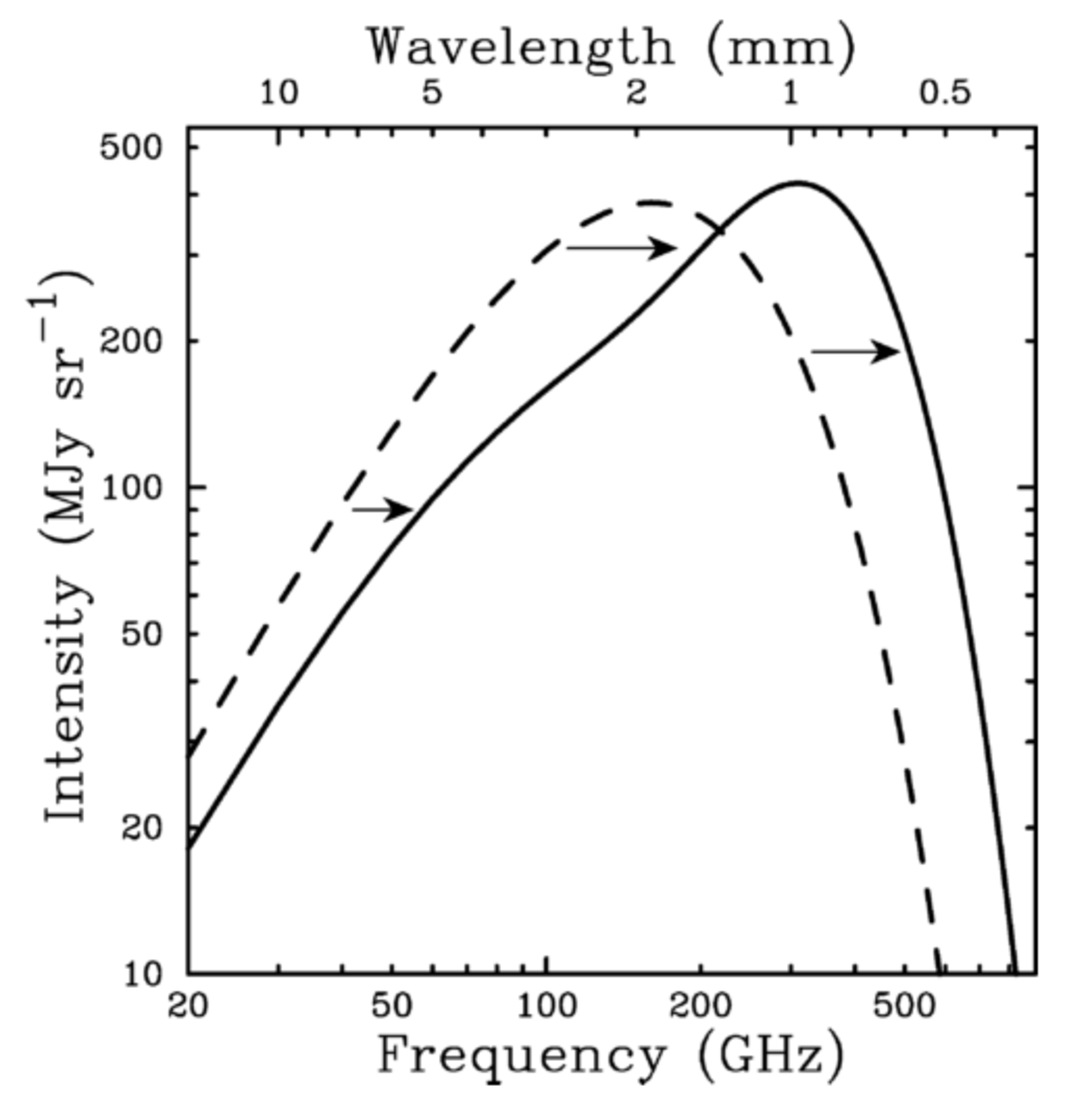
\includegraphics[height=0.5\textheight]{figures/sze.pdf}
	\end{center}
	\caption[The Sunyaev-Zel'dovich Effect.]{Adapted from \cite{Carlstrom2002a}, the undistorted CMB spectrum (dashed line) is shifted to a higher energy (solid line) by the SZE. Note: this shift is for illustration purposes only, the SZE distortion shown is for a fictional cluster 1000 times more massive than a typical massive galaxy cluster.}
	\label{fig:sze}
\end{figure}
High resolution images of the CMB can detect a ``hole'' in the CMB at frequencies below 218 GHz, and a bright spot at higher frequencies due to the shift in the CMB black body spectrum. The temperature of the ICM effects the shift in the CMB frequency. Therefore the shift depends on cluster mass and therefore SZE cluster studies provide a means to test cosmological parameters \citeeg{Bocquet2015, DeHaan2016}. 

At their completion, the South Pole Telescope (SPT; \citealt{Carlstrom2011}) and the Atacama Cosmology Telescope (ACT; \citealt{Swetz2011}) are expected to find approximately one thousand clusters using observations in the millimeter combined with the SZE. Attempts are already underway to calibrate these observations using subsamples of clusters (approximately 100 cluster candidates and 60 clusters respectively) and other observables such as optically-based, virial estimates or X-ray temperature measurements \citeeg{Sifon2013, Bocquet2015}. 

\subsection{Optical}
Clusters of galaxies have been historically identified as over-densities of galaxies detected in their optical light \citeeg{Abell1958}, and the dynamics of their constituent galaxies can be used to estimate their virial masses. Much like the X-ray observations, the motions of the individual member galaxies (referred to as velocity dispersion) provide an estimate of the depth of the cluster's gravitational potential well, which is an estimate of the total cluster mass. The constituent cluster galaxies act as tracer particles through the cluster's potential well. This can be modeled in simulations and has been the focus of many recent studies \citeeg{Evrard2008, Munari2013, Saro2013, Sifon2013, VanderBurg2014}. This type of measurement is important because it is independent of the physics of the ICM, which are always not fully understood. However, these measurements require spectroscopy, which is expensive to obtain.

\begin{figure}[!ht]
	\begin{center}
		%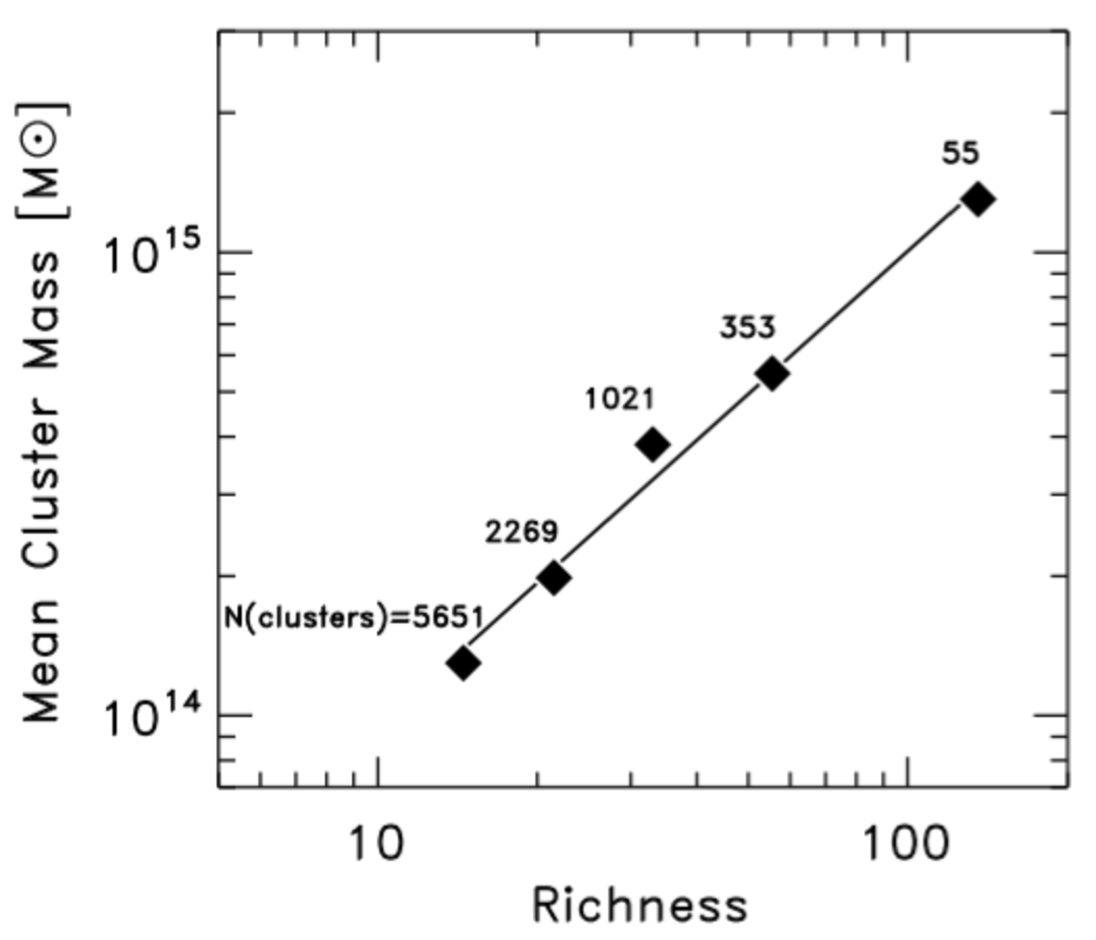
\includegraphics[width=0.6\textwidth]{figures/massrichness.pdf}
		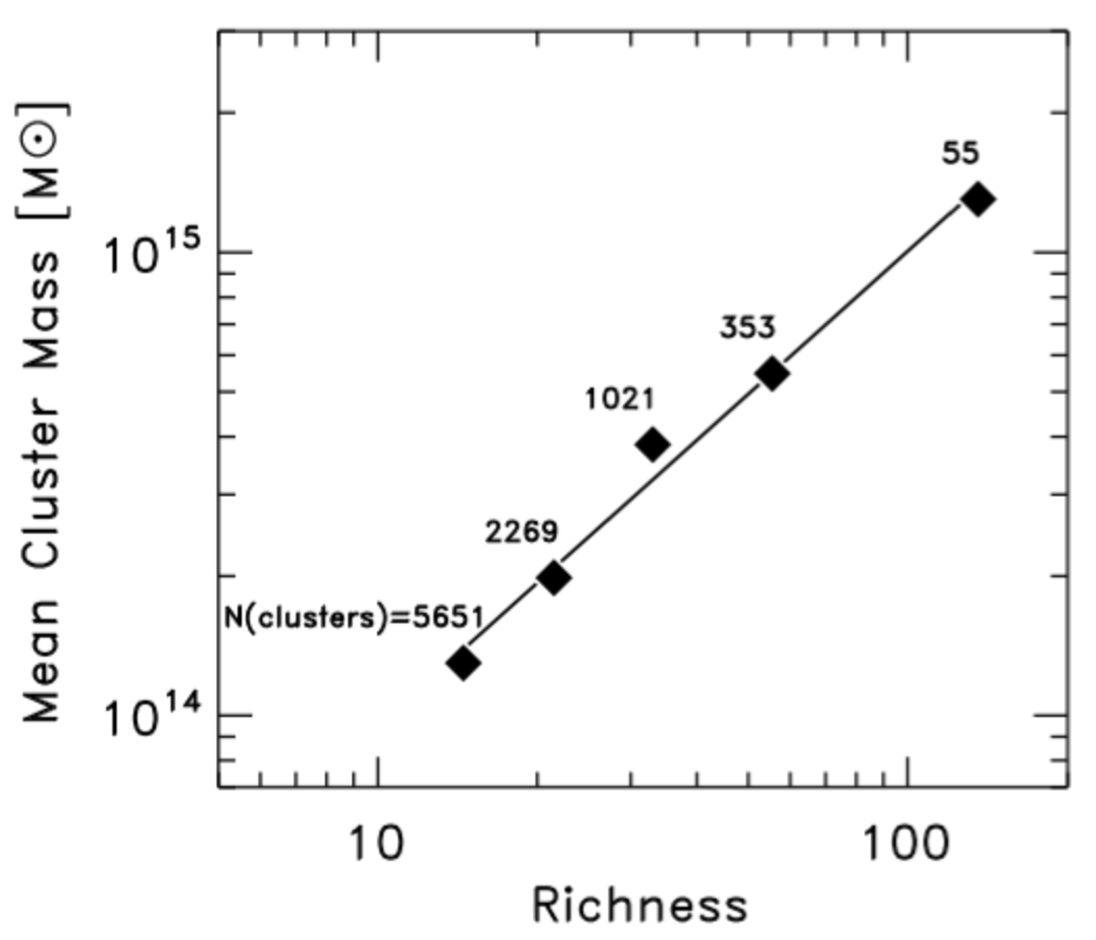
\includegraphics[height=0.5\textheight]{figures/massrichness.pdf}
	\end{center}
	\caption{The relation between the mean Richness and the mean cluster mass.} 
	Derived from stacked weak lensing measurements and adapted from \citealt{Rozo2010}, the number of clusters in each stack are given above each data point. There is a strong correlation between richness and cluster mass, however, because the data are stacked, the absolute mass scale and scatter in mass at fixed richness are imprecisely known.
	\label{fig:massrichness}
\end{figure}

It is possible to estimate both cluster membership and mass through photometric observations alone, using modern cluster finding algorithms such as the red-sequence Matched-Filter Probabilistic Percolation (redMaPPer; \citealt{Rykoff2014}) method which measures a galaxy cluster's richness, $\lambda$. The richness measurement, in the case of redMaPPer, is a probability weighted cluster membership, where the probability is whether or not an individual galaxy belongs to the cluster in question. Figure~\ref{fig:massrichness} shows the richness correlates strongly with cluster mass on average \citeeg{Rozo2010}, but the absolute mass scale of the optical richness mass estimator and the scatter in cluster mass at fixed optical richness are imprecisely known \citep{Rykoff2012}.

The Dark Energy Survey (DES; \citealt{DES2005}) will survey 5000 \degsq\ of the southern sky and is expected to detect 100,000 clusters at $z<1$ \citep{DarkEnergySurveyCollaboration2016}. The Large Synoptic Survey Telescope (LSST; \citealt{LSST2012}) will also survey an enormous portion of the southern sky, extremely deeply and will identify vast numbers of clusters using optical selection methods \citeeg{Rykoff2014, Rozo2014}. However, these surveys will be photometric, and any spectral information will be obtained from preexisting datasets. While it is possible to estimate cluster masses using photometric observations, primarily through the richness-mass relation. Because the primary goal is to have reliable cluster mass estimates, multiple mass-checking observations are required. The spectroscopic calibration of the optical richness-mass relation provided by HETDEX is required to both better calibrate the relation and to obtain the level of precision needed to compete with other mass estimators.

\section{Cluster Formation: Relationship to Cosmological Parameters}
Thought to form out of the primordial density fluctuations in the very early Universe, galaxy cluster formation and growth investigations began in the 1960s \citeeg{VanAlbada1960, VanAlbada1961}. Soon thereafter, the hierarchical model of structure formation \citep{Press1974, Gott1975, White1978} was introduced. It suggests the first stars and stellar clumps formed then subsequently merged together with DM and other gas clumps to form the first galaxies which then continued to merge and grow into the clusters and large scale structures we see today. In this model, structures grow through the accretion of smaller systems through the gravity of the DM associated with the cluster. Of course, many complicated astrophysical processes are at work during cluster growth \citeeg{Boschin2004, DeLucia2007a} and similarly complicated theoretical models seek to explain these processes. For a detailed review of cluster formation see \cite{Kravtsov2012}.

Because their initial seeds were planted in the very early Universe, the number and distribution of galaxy clusters across the sky are the fingerprints of the cosmology imprinted on the Universe at its birth. Therefore, measuring a census of cluster properties, such as mass, provides a strong constraint on the cosmological parameters \citeeg{Benson2013, Mantz2015, DeHaan2016}; see Subsection~\ref{sec: GC Cosmology}. The study of galaxy clusters stand at the intersection of cosmology and astrophysics. 

\section{Cosmology with Galaxy Clusters}\label{sec: GC Cosmology}
The current concordance cosmology is a parametrization of the Big Bang cosmological model where the Universe contains a cosmological constant ($\Lambda$; often referred to as dark energy) and cold dark matter (CDM). It is often characterized by six parameters; the Hubble Constant ($H_0$), the baryonic matter density ($\Omega_b$), the DM density ($\Omega_c$), the dark energy density ($\Omega_\Lambda$); the normalization of the power spectrum ($\sigma_8$); and the spectral index of the power spectrum ($n_s$). 

Galaxy clusters are sensitive probes of $\Omega_m$, the total mass ($\Omega_b + \Omega_c$) density in the Universe and $\sigma_8$. Galaxy clusters trace the peaks in the universal matter density, often referred to as the power spectrum of matter density fluctuations or the matter power spectrum, much in the same way islands (mountain peaks) trace land masses through the earth's oceans. We can constrain the values of $\Omega_m$ and $\sigma_8$ by comparing the number density of the observed galaxy clusters to that predicted by cosmological models.

The determination of cosmological parameters is done by comparing the number of galaxy clusters per unit mass per unit comoving volume ($n(M,z)$) to models. See \cite{Allen2011} for a comprehensive review or \cite{Murray2013} for a more practical approach. $n(M,z)$, referred to as the halo mass function (HMF) captures the number evolution through a function which defines the particular model used \citeeg{Tinker2008}. Early work by \cite{Press1974} and \cite{Bond1991} which assumed spherically symmetric halos, has largely been replaced by more modern fitting functions which, at the expense of an analytical solution, provide more accurate results when fit to simulation data. See \cite{Murray2013} for a review of the most common fitting functions used. Through this approach, the two parameters which clusters are most sensitive to, $\Omega_m$ and $\sigma_8$, are in reality measured as $\sigma_8\Omega_m^\alpha$, where the value of $\alpha$ depends on the masses of the halos considered. The degeneracy is broken through the evolution of the HMF as a function of redshift. 

The accuracy of the estimates of $\Omega_m$ and $\sigma_8$ depends on how well the observed HMF can be measured. The correctness of the HMF depends directly on the number of galaxy clusters observed and the accuracy to which the mass of each of the clusters can be estimated. As we discuss below, the identification of large numbers of clusters is not a considerable contributing factor to the uncertainty; the total number of clusters known is only increasing. The accurate recovery of galaxy cluster mass for both very rich clusters (those with high mass) and, importantly, the poor clusters (those with low mass) remains the dominate source of uncertainty \citeeg{Sehgal2011,Plank2014, Bocquet2015}.

\section{Galaxy Cluster Surveys as a Data Science Challenge}
Astronomy and astrophysics are undergoing a data revolution. Advances in telescope design, detectors, and computing resources have provided more astronomical data than any previous time in the history of the field. Beginning in the early 2000s, astronomical surveys have generated many hundreds of terabytes of data for many millions of sources. In the coming years, this data excess will grow beyond the terabyte regime with observations of billions of astronomical objects. 

The all-sky X-ray survey conducted by eROSITA is expected to identify 50,000 or more clusters. SPT and ACT are discovering many thousands of clusters through the SZE. DES and LSST will optically identify many tens of thousands of clusters with much lower masses than are possible with SZE measurements. Taken together, these surveys will produce data products which are both immense and heterogeneous. The multi-wavelength observations ensures there will be many observational parameters associated with each cluster. However, different observation wavelengths probe different cluster physics making them more or less sensitive probes of a specific galaxy cluster's total mass. Varying angular resolutions will also play a role as the instruments used to collect the data will observe in a wide range of wavelength and be both ground and space based. Therefore, the combination of datasets will be a significant challenge, and the goal of this thesis is to tackle one of these challenges.

The ability to associate individual or combinations of observations with the cluster property in question will be a powerful statistical tool. For example, training machine learning algorithms on a wide range of cluster properties (velocity dispersion, richness, redshift, etc.) could potentially produce more accurate estimates of cluster mass with smaller scatter. This is a question we will attempt to address over the next two chapters. 

\subsection{Machine Learning}
Machine learning (ML) is a branch of computer science focused on the study and construction of computational tools which can learn from and make predictions based on data. In 1959, Arthur Samuel (December 5, 1901 -- July 29, 1990), an early computer gaming pioneer, described ML as a ``field of study that gives computers the ability to learn without being explicitly programmed'' \citep{simon2013}. While, a great deal of programming is often required (discussed further below), such algorithms work by comparing data to a set of models allowing them to make predictions based on the data rather than preprogrammed commands.

ML can be broken into two large categories, unsupervised or supervised learning. ``Unsupervised learning'' is where the ML algorithm is tasked to make qualitative statements about the structure of unlabeled data. An example would be finding clusters of data inside a large dataset, where the number and location of the clusters are not known a priori (\eg, locating galaxy clusters in observations of galaxy positions; see Section~\ref{sec: future}). ``Supervised learning'' \citeeg{mohri2012} asks the computer to make predictive statements about one variable based on labeled observations of another or combination of other variables. An example could be photometric redshift prediction; given a large number of color and magnitude measurements for a galaxy, predict the most probable redshift.  

In this thesis, we are concerned with supervised learning, where we know a relationship exists between two sets of data, and we use a computer algorithm to infer the relationship for us. The algorithm uses a decision tree to learn which works by mapping a set of observations (``features'') of a source to a set of conclusions (``targets'') about that source. If the set of conclusions is finite, then the method becomes a classification tree; if the conclusions are infinite then it becomes a regression tree. 

\begin{figure}[!ht]
	\begin{center}
		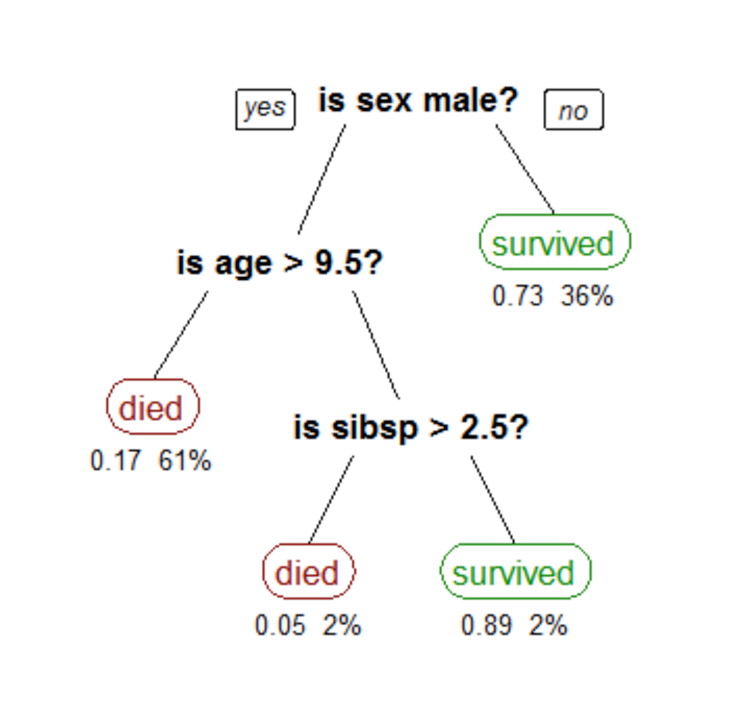
\includegraphics[height=0.5\textheight]{figures/CART_tree_titanic_survivors.pdf} 
	\end{center}
	\caption[An example of a classification tree.]{Decision tree classifying the survival of passengers on the RMS Titanic. ``sibsp'' represents the number siblings or spouses aboard, and the numbers below each class represents the probability of survival and fraction of passengers which are classified into each leaf. Credit: Stephen Milborrow (Own work) [CC BY-SA 3.0 or GFDL]}
	\label{fig: cart tree} 
\end{figure}

Figure~\ref{fig: cart tree} shows a simple example of a classification tree for the survivability of passengers on the RMS Titanic. The bolded text is referred to as interior nodes which correspond to a single feature of each passenger in the example, sex, age and number of siblings or spouses. The ending points are called leaves which represent the value of the target variable given the value of the features input into the tree. For this example, there are two possible ending leaves, ``died'' or ``survived.'' Using this simple tree we are able to classify all passangers into the two possible classes. 

The ML algorithm ``learns'' this tree by choosing a feature from all available features which best separates the input data into two or more subsets. In the case of the example, this is the sex of the passenger. This becomes the root node. All subsequent nodes are created by repeating this process on each subset associated with the previous node. In such manner, it will split the male passengers by age and then by number of siblings for the males older than 9.5 years. This process is known as a top-down induction of decision trees and is the most common method for creating decision trees from data.

Once the decision tree has been learned, it can be used to classify data not seen before. For example, a 30 year-old, male passenger of the RMS Titanic has a probability of survival of 17\% and so will most likely be classified as ``died'' by the ML algorithm. However, imagine for a moment, with the benefit of hindsight that we know this male passenger survives. Only 17\% of the time will the ML method classify the passenger as ``survived'' based on this decision tree. We can boost the predictive power of the tree by generating many trees and then combining the final predictions at the end. Methods that construct more than one tree are called ensemble methods. For this thesis, we use an ensemble method know as a forest of randomized trees and discuss them further in Section~\ref{sec:machine learning method} and Section~\ref{2sec:ML based cluster masses}.

\section{This Work}
The goal of this thesis is to understand how a survey such as the Hobby Eberly Dark Energy Experiment (HETDEX; \citealt{Hill2008}) can reduce the associated systematic uncertainties of galaxy cluster mass scaling relations, specifically the scatter in the optical richness-cluster mass scaling relation. The relationship between cluster observable and the cluster mass is often noisy and includes large systematic uncertainties \citeeg{Rozo2013, Sereno2015}. It is because of these reasons that the dominant source of uncertainty in deriving cosmological constrains from galaxy clusters is the systematic uncertainty associated with the cluster mass estimates \citeeg{Vikhlinin2009, Rozo2010, Mantz2015}.

There are two systematic uncertainties present in the optical richness-cluster mass scaling relation: the absolute mass scale is the predicted cluster mass for a give richness, and the scatter ($\sigma$) of observed cluster masses ($M$) at fixed optical richness ($\lambda$), $\sigma_{M|\lambda}$. The absolute mass scale can be well calibrated with studies utilizing stacked cluster data \citeeg{Baxter2016, Farahi2016, Simet2016} where many cluster measurements are combined to decrease the uncertainty associated with the mass measurement. However, such studies cannot well constrain $\sigma_{M|\lambda}$ because any mass scatter is lost during the stacking process. Understanding, constraining, and ultimately reducing $\sigma_{M|\lambda}$ is paramount to the accurate estimates of cosmological parameters, and an accurate measure of this scatter can lead to a decrease on the error bar on cosmological measures sensitive to cluster abundances ($\sigma_8$ and $\Omega_m$) by as much as 50\% \citep{Rozo2010}.

At present, few studies have attempted to characterize $\sigma_{M|\lambda}$ \citep{Rozo2014,Rozo2015, Saro2015, Rykoff2016}. This is due, in large part, to the lack of availability of large-area sky surveys capable of providing the accurate cluster mass estimates for single galaxy clusters required to measure $\sigma_{M|\lambda}$. As we discussed previously, this is quickly changing as new large-area sky surveys across a multitude of wavelengths are detecting many thousands of galaxy clusters. 

This thesis seeks to investigate the the ability of HETDEX to better constrain $\sigma_{M|\lambda}$. HETDEX is a forthcoming large-area blind spectroscopic sky survey with a primary science mission of measuring the dark energy equation of state at $z\sim2$. As such, the applicability to galaxy cluster science has not yet been investigated. In addition, because the survey is blind, it will detect nearly as many galaxies at $z<0.5$ as it will at $z>2.$ Therefore, HETDEX is an enormous, potentially useful dataset for cosmology science using galaxy clusters, but this has not yet been explored. This is a primary goal of this thesis. We discuss HETDEX further in Section~\ref{sec: hetdex}.

In Chapter 2, we first use a set of state-of-the-art simulations where we replicate the observing strategy of HETDEX to determine the number and nature of clusters that might be observed. This is accomplished in two ways; in each part we measure the cluster properties, such as redshift, velocity dispersion, and mass of the clusters. First we use targeted observations and perfect knowledge of the observed galaxy clusters, which includes center, membership, and number to recover the desired properties. Secondly, we assume that we know the location, but not the center, membership, or number of constituent galaxies. Then we will employ the HETDEX observing strategy, including realistic pointing pattern, observational magnitude constraints, and spectral sensitivity limits to generate a set of realistic observations.

For the two sets of observations, we use three methods to estimate each galaxy cluster's mass; a traditional power law scaling relation between the observed line-of-sight velocity dispersion and the cluster mass, a probability based method which attempts to combine additional observables with the line-of-sight velocity dispersion, and a ML based approach which also uses multiple observables. Then, using those cluster mass estimates, we attempt to characterize the optical richness-cluster mass relation to better understand the amount of intrinsic scatter when using HETDEX like observations. This enables us to more fully understand and contrain the HMF which, in turn, allows us to make more accurate measurements of $\sigma_8$ and $\Omega_m$.

In Chapter 3 of this thesis, we describe a practical test of the approaches we develop in the simulation-based portion of this thesis, we use targeted integral field unit spectroscopic observations of ten intermediate redshift clusters with the Mitchell Spectrograph (formerly known as VIRUS-P; \citealt{Hill2008a}), the prototype instrument for HETDEX. Using the spectra obtained for the galaxies associated with each cluster, we determine the cluster membership, determine the cluster mass using the line-of-sight velocity dispersion-cluster mass scaling relation from before, and also combine cluster observables through ML to predict the cluster masses. We again estimate $\sigma_{M|\lambda}$ for the observed clusters.

Finally, in Chapter 4 of this thesis we summarize the main results of this work. In addition, we outline some prospects for future investigations with the HETDEX dataset, and discuss outstanding questions that remain. 
